%% LyX 2.3.6.1 created this file.  For more info, see http://www.lyx.org/.
%% Do not edit unless you really know what you are doing.
\documentclass[english]{article}
\usepackage[T1]{fontenc}
\usepackage[latin9]{inputenc}
\usepackage{geometry}
\geometry{verbose,lmargin=1cm,rmargin=1cm}
\usepackage{amstext}
\usepackage{graphicx}
\PassOptionsToPackage{normalem}{ulem}
\usepackage{ulem}

\makeatletter

%%%%%%%%%%%%%%%%%%%%%%%%%%%%%% LyX specific LaTeX commands.
%% Because html converters don't know tabularnewline
\providecommand{\tabularnewline}{\\}

\makeatother

\usepackage{babel}
\begin{document}
\title{Homework 3}
\author{Antonio Zea Jr}
\maketitle

\section{Consider the following languages:}

\subsection*{$L_{1}=\{w|w\in\{a,+,-,*,/,(,)\}^{*},w\text{ is a legal arithmetic expression in infix form}\}$}

\subsection*{$L_{2}=\{w|w\in\{0,1\}^{*},w\text{ contains at least three 1s}\}$}

\subsection*{$L_{3}=\{w|w\in\{0,1\}^{*},w\text{ the length of w is odd}\}$}

\subsection*{$L_{4}=\{w|w\in\{0,1\}^{*},w\text{ starts and end with the same symbol}\}$}

\subsection*{$L_{5}=\{w|w\in\{0,1\}^{*},w\text{is a palindrome}\}$ }

\subsection*{$L_{6}=\{w|w\in\{0,1\}^{*},w\text{contains equal numbers of 0s and 1s}\}$}

\section{Which languages are regular and which are not? Give the \uline{regular
expressions} for the regular languages.}

\subsection*{$L_{1}$ is nonregular}

\subsection*{$L_{2}=10^{*}10^{*}1(0\cup1)^{*}$}

\subsection*{$L_{3}=((0\cup1)(0\cup1))^{*}(0\cup1)$}

\subsection*{$L_{4}=0(0\cup1)^{*}0\cup1(0\cup1)^{*}1$}

\subsection*{$L_{5}$ is nonregular}

\subsection*{$L_{6}$is nonregular}

\section{For each nonregular language prove that it is not regular by using
the pumping lemma or the closure of the regular languages.}

\subsection*{$L_{1}=\{w|w\in\{a,+,-,*,/,(,)\}^{*},w\text{ is a legal arithmetic expression in infix form}\}$}

Assume $L_{1}$ is regular, then there is a number $p$ (pumping length)
where if $s$ is any string in $L_{1}$ of length at least $p$, then
$s$ may be divided into three pieces, $s=xyz$, satisfying the following
conditions:

1. $\forall i\geq0$ , $xy^{i}z\in L_{1}$

2. $|y|>0$

3. $|xy|\leq p$\\
Let $s=(a+a)$

case 1: y is in the first set 

\subsection*{$L_{5}=\{w|w\in\{0,1\}^{*},w\text{is a palindrome}\}$ }

Assume $L_{5}$ is regular, then there is a number $p$ (pumping length)
where if $s$ is any string in $L_{1}$ of length at least $p$, then
$s$ may be divided into three pieces, $s=xyz$, satisfying the following
conditions:

1. $\forall i\geq0$ , $xy^{i}z\in L_{1}$

2. $|y|>0$

3. $|xy|\leq p$\\
Let $s=w(0\cup1\cup\varepsilon)w^{\mathcal{R}}$somehow $s=xyz$

case 1: $y$occurs in $w$

case 2: $y$occurs in $w^{\mathcal{R}}$

case 3: $y$ occurs inbetween with part

\subsection*{$L_{6}=\{w|w\in\{0,1\}^{*},w\text{contains equal numbers of 0s and 1s}\}$}

\section{For each language \uline{give the CFG} that describes it.}

\subsection*{$L_{1}=\{w|w\in\{a,+,-,*,/,(,)\}^{*},w\text{ is a legal arithmetic expression in infix form}\}$}

CFG

$S\rightarrow a|SXS|(SXS)$

$X\rightarrow+|-|*|/$

\subsection*{$L_{2}=\{w|w\in\{0,1\}^{*},w\text{ contains at least three 1s}\}$}

CFG

$S\rightarrow X1X1X1X$

$X\rightarrow0X|1X|\varepsilon$

\subsection*{$L_{3}=\{w|w\in\{0,1\}^{*},w\text{ the length of w is odd}\}$}

CFG

$S\rightarrow0X|1X$

$X\rightarrow0S|1S|\varepsilon$

\subsection*{$L_{4}=\{w|w\in\{0,1\}^{*},w\text{ starts and end with the same symbol}\}$}

CFG

$S\rightarrow0X0|1X1|\varepsilon$

$X\rightarrow0X|1X|\varepsilon$

\subsection*{$L_{5}=\{w|w\in\{0,1\}^{*},w\text{is a palindrome}\}$ }

CFG

$S\rightarrow0S0|1S1|0|1|\varepsilon$

\subsection*{$L_{6}=\{w|w\in\{0,1\}^{*},w\text{contains equal numbers of 0s and 1s}\}$}

CFG

$S\rightarrow SS|0S1|1S0|\varepsilon$

\section{Use the \uline{CFG Developer} to \uline{test the grammars}
for all languages. Try strings that belong to the language of the
grammar and strings that do not. Show the derivations of the strings
that belong to the language.\protect \\
\begin{tabular}{|c|c|}
\hline 
 & \tabularnewline
\hline 
\hline 
 & \tabularnewline
\hline 
\end{tabular}

$L_{1}$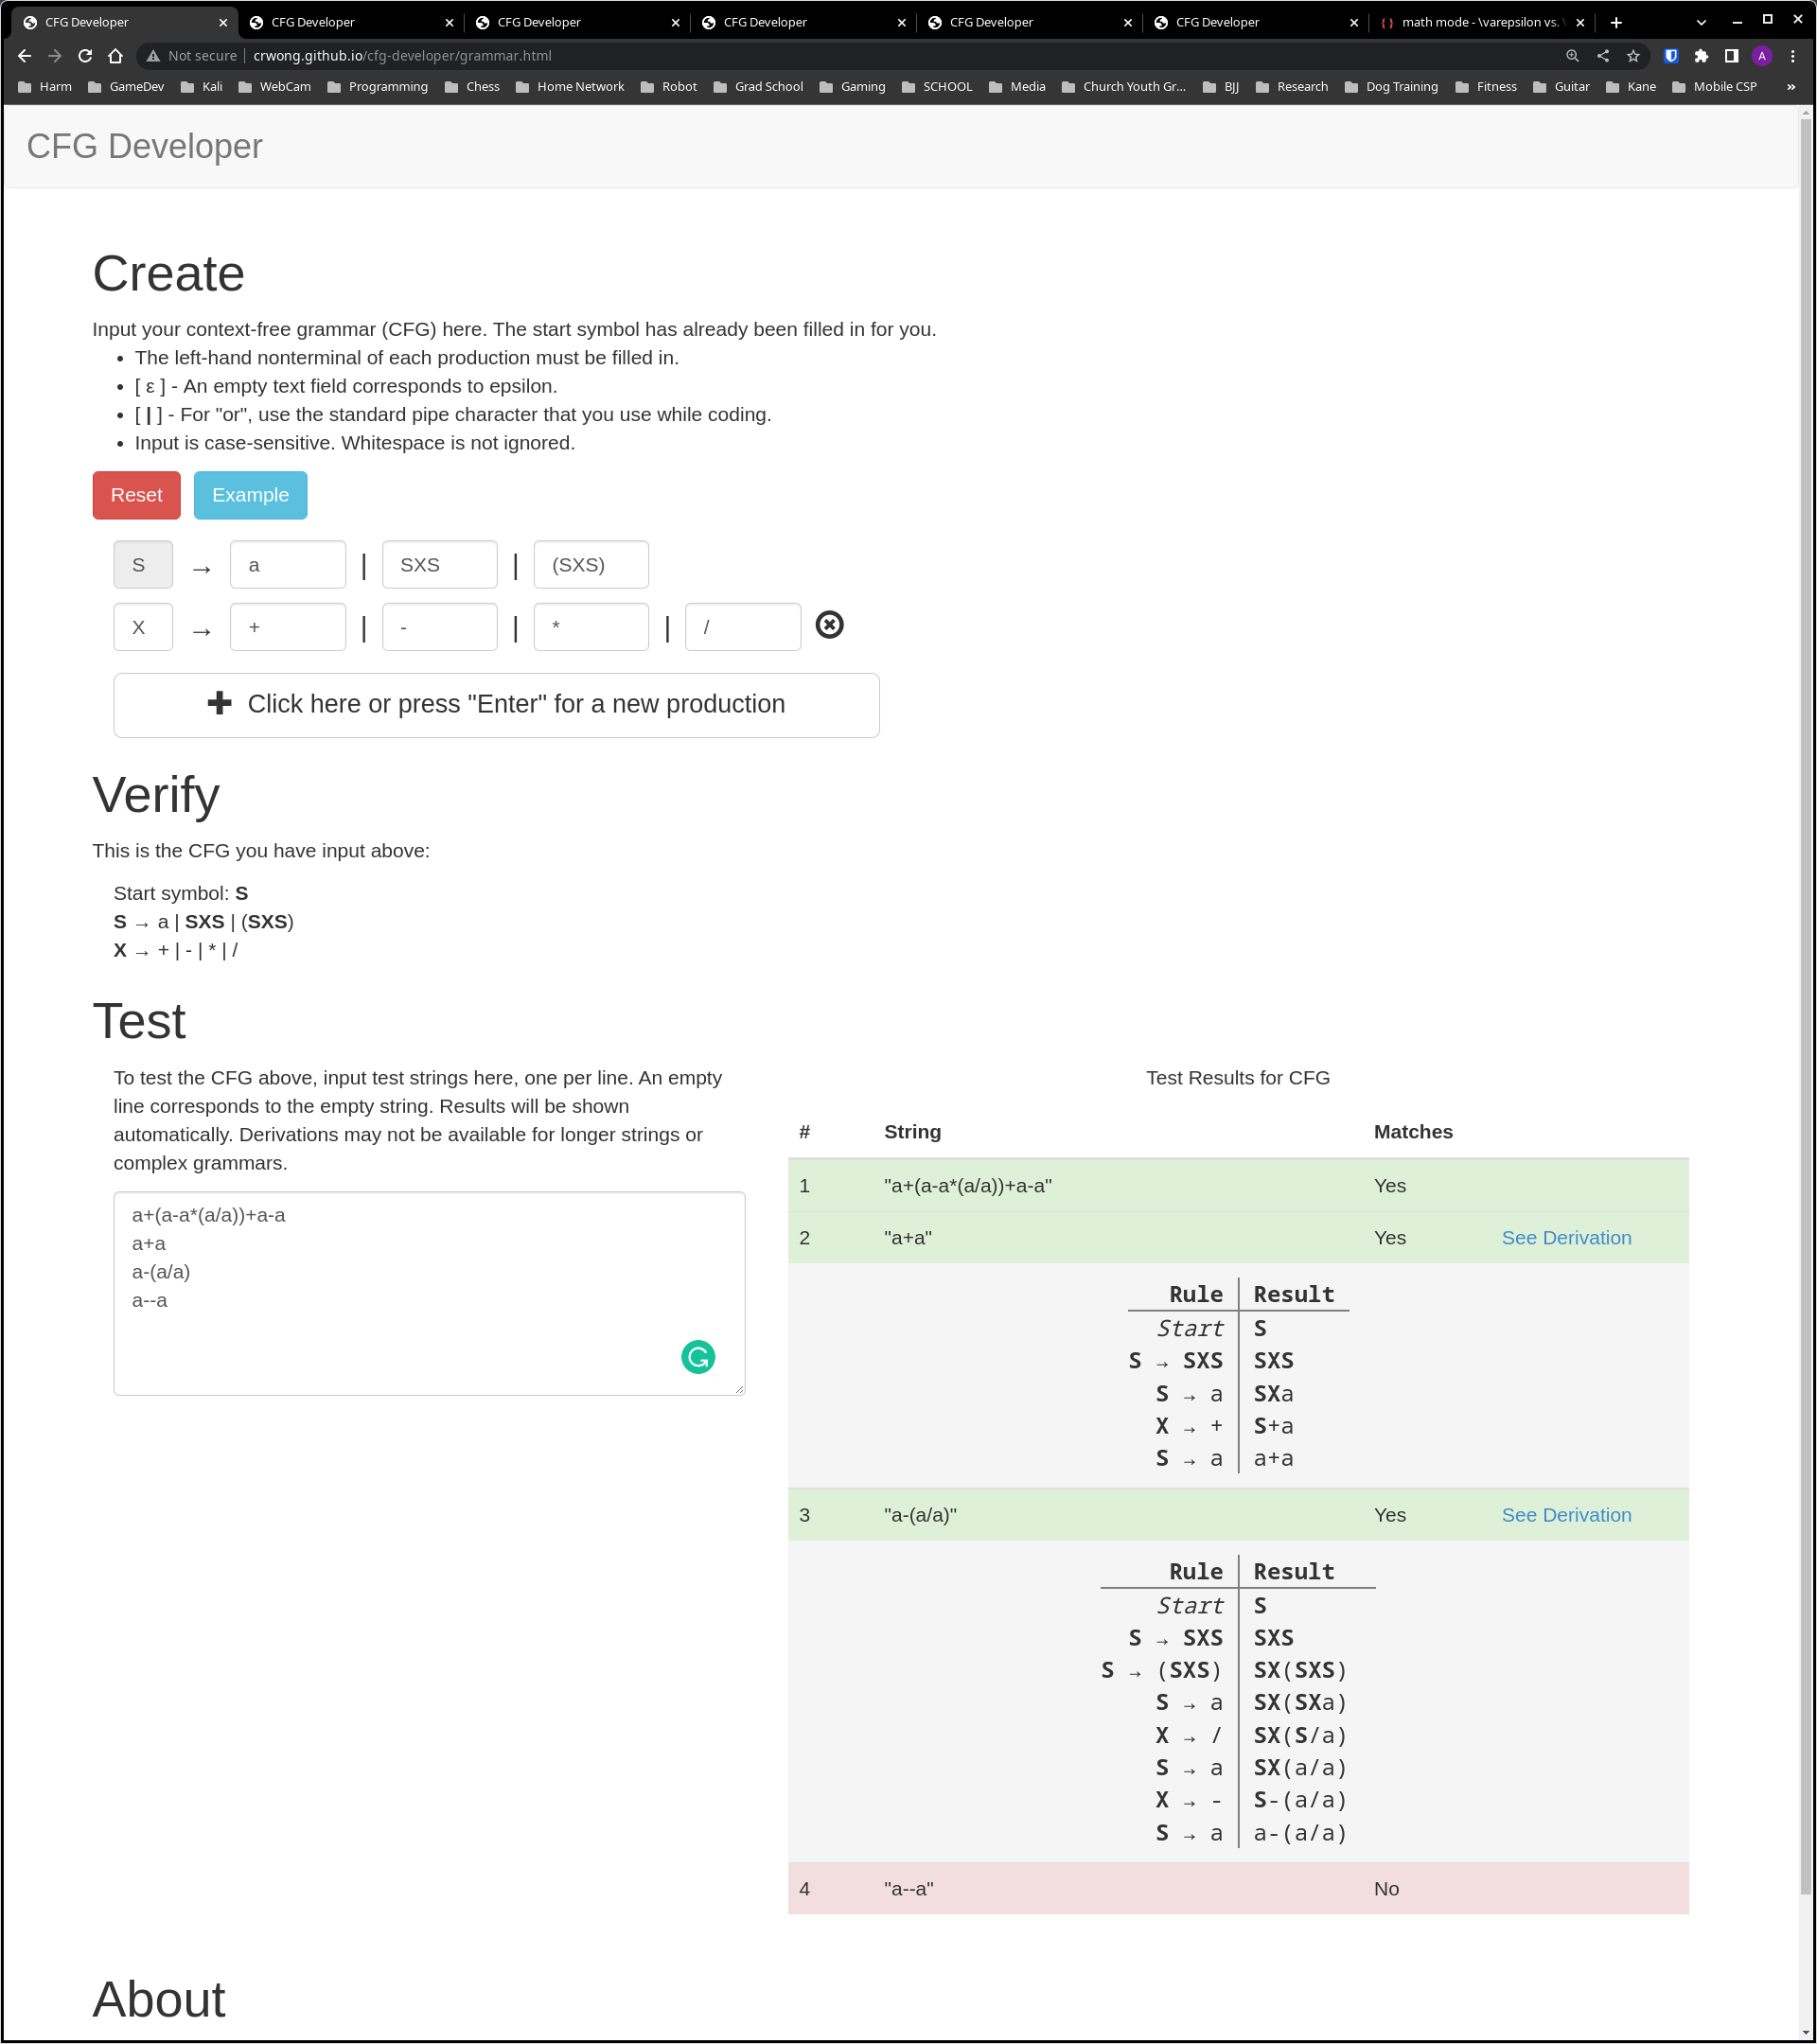
\includegraphics[width=0.4\paperwidth]{cfg_l1}\\
$L_{2}$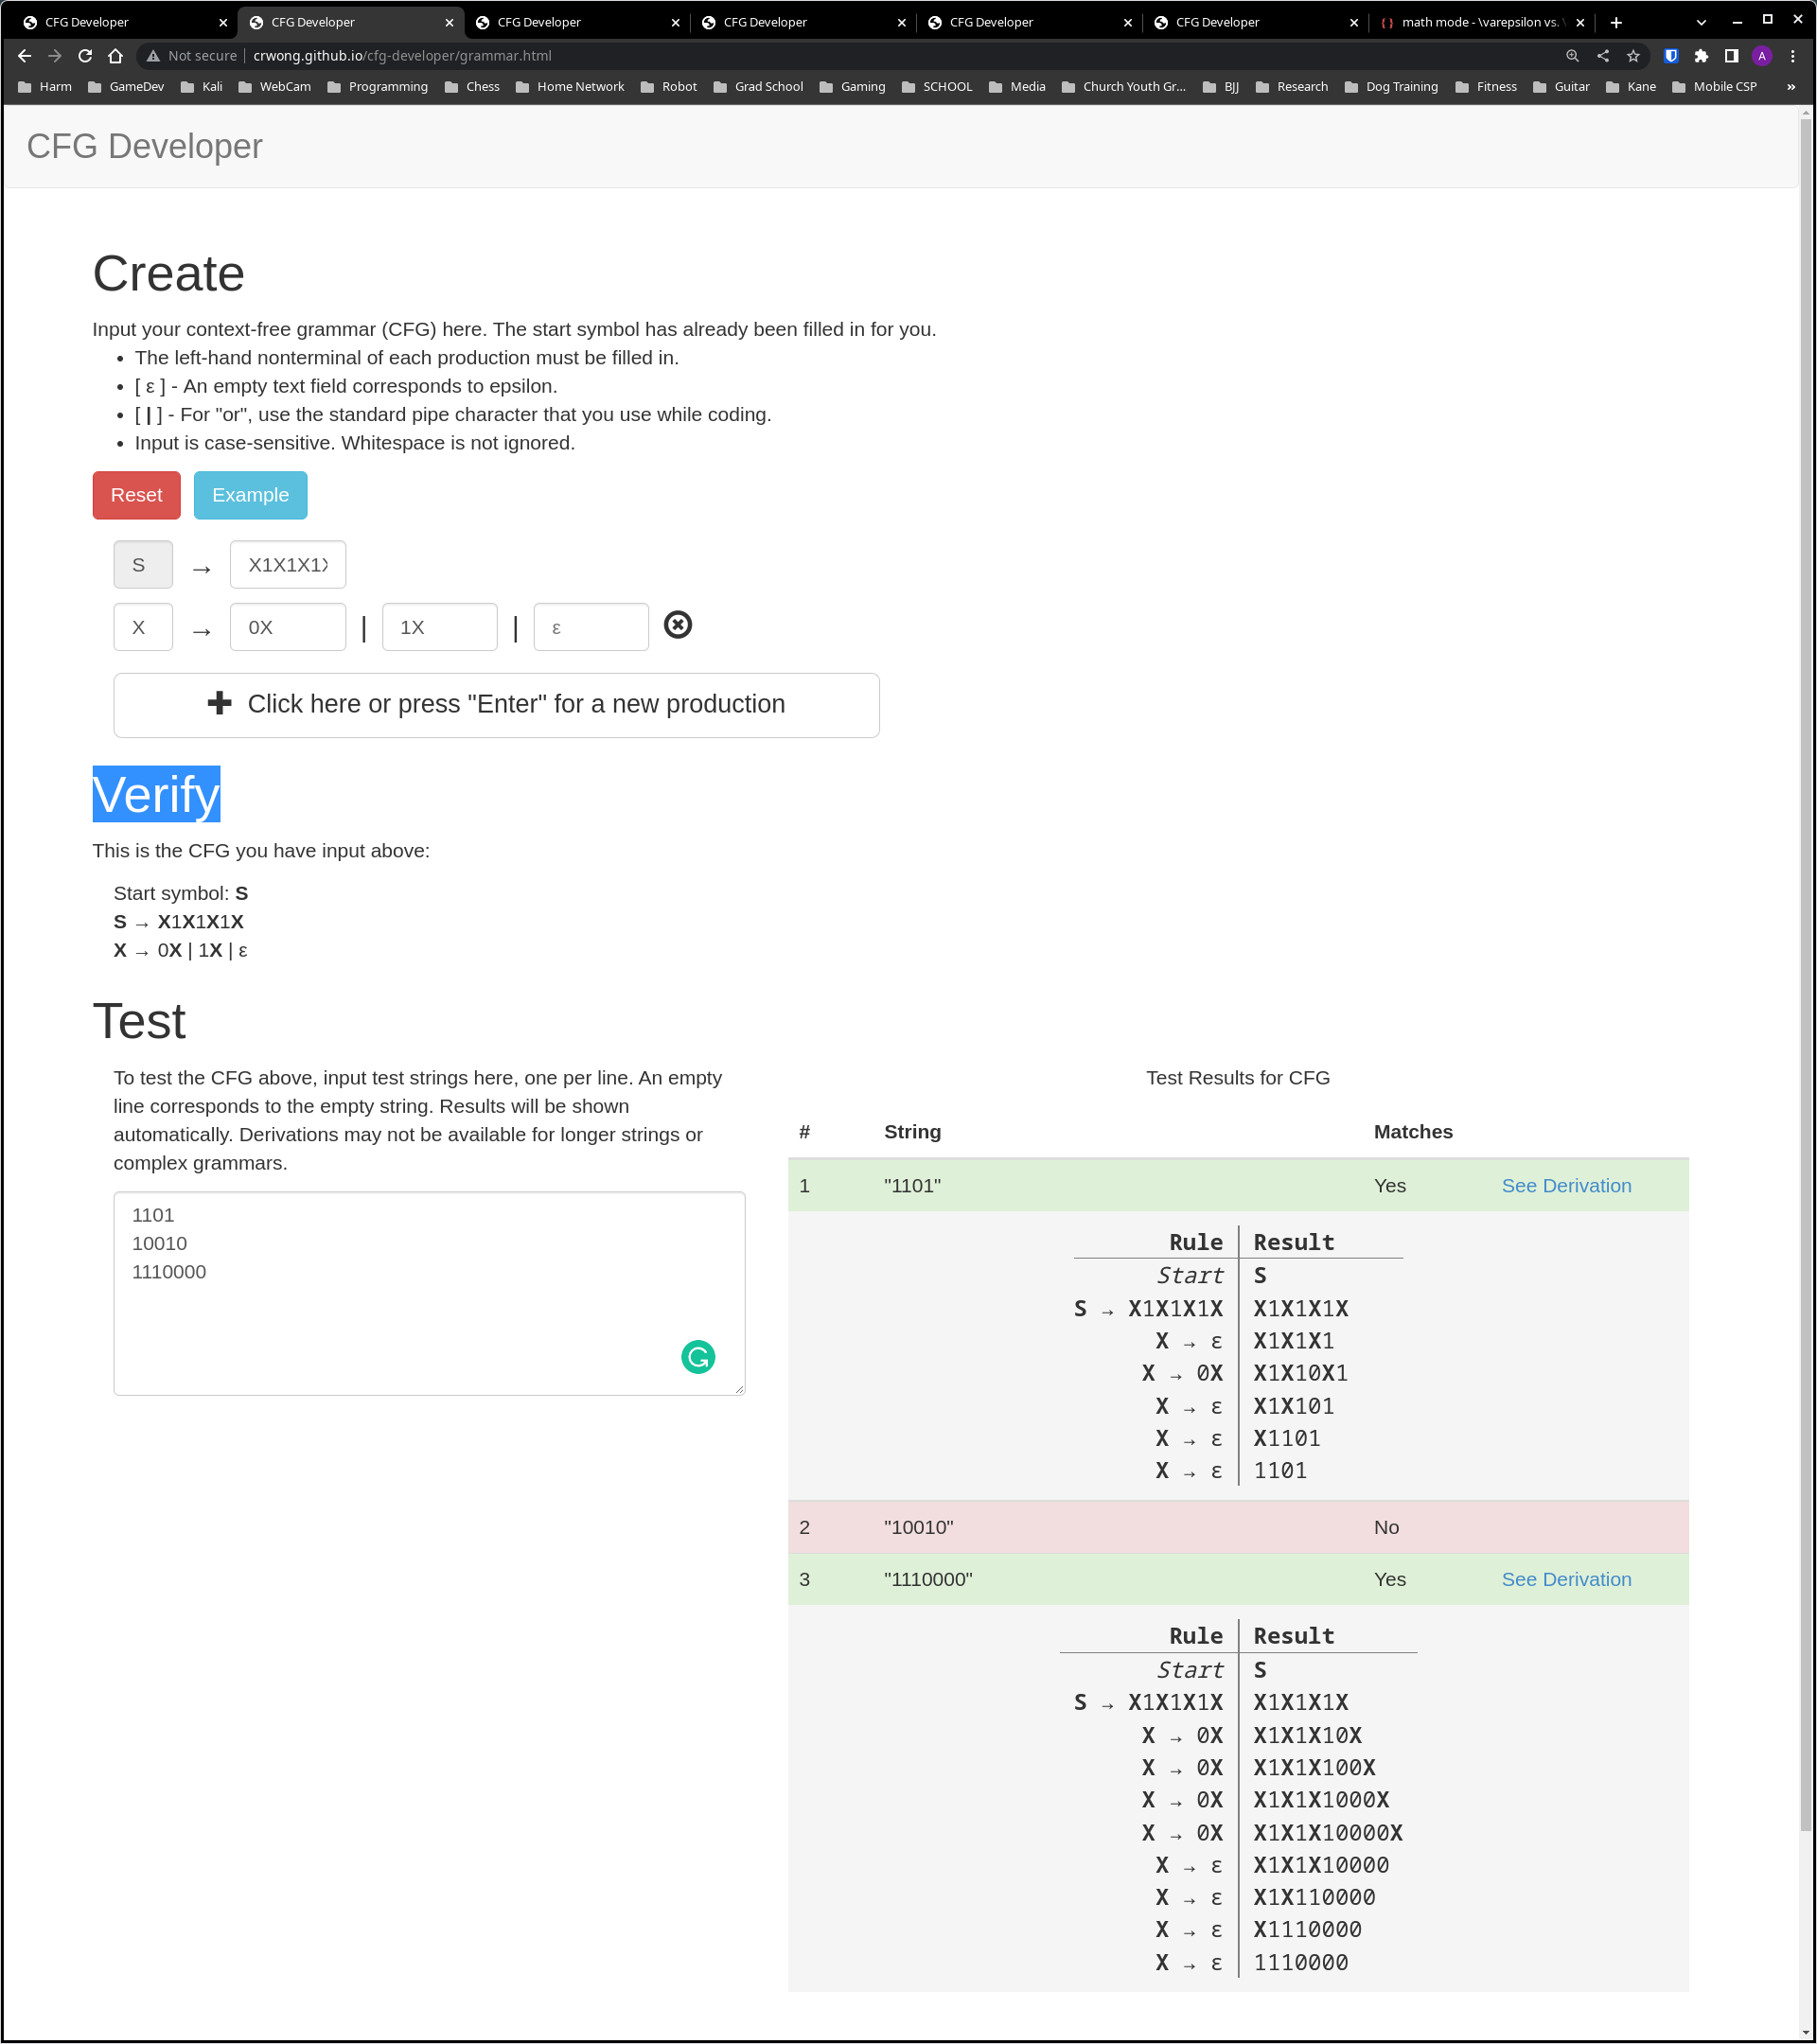
\includegraphics[width=0.4\paperwidth]{cfg_l2}\\
$L_{3}$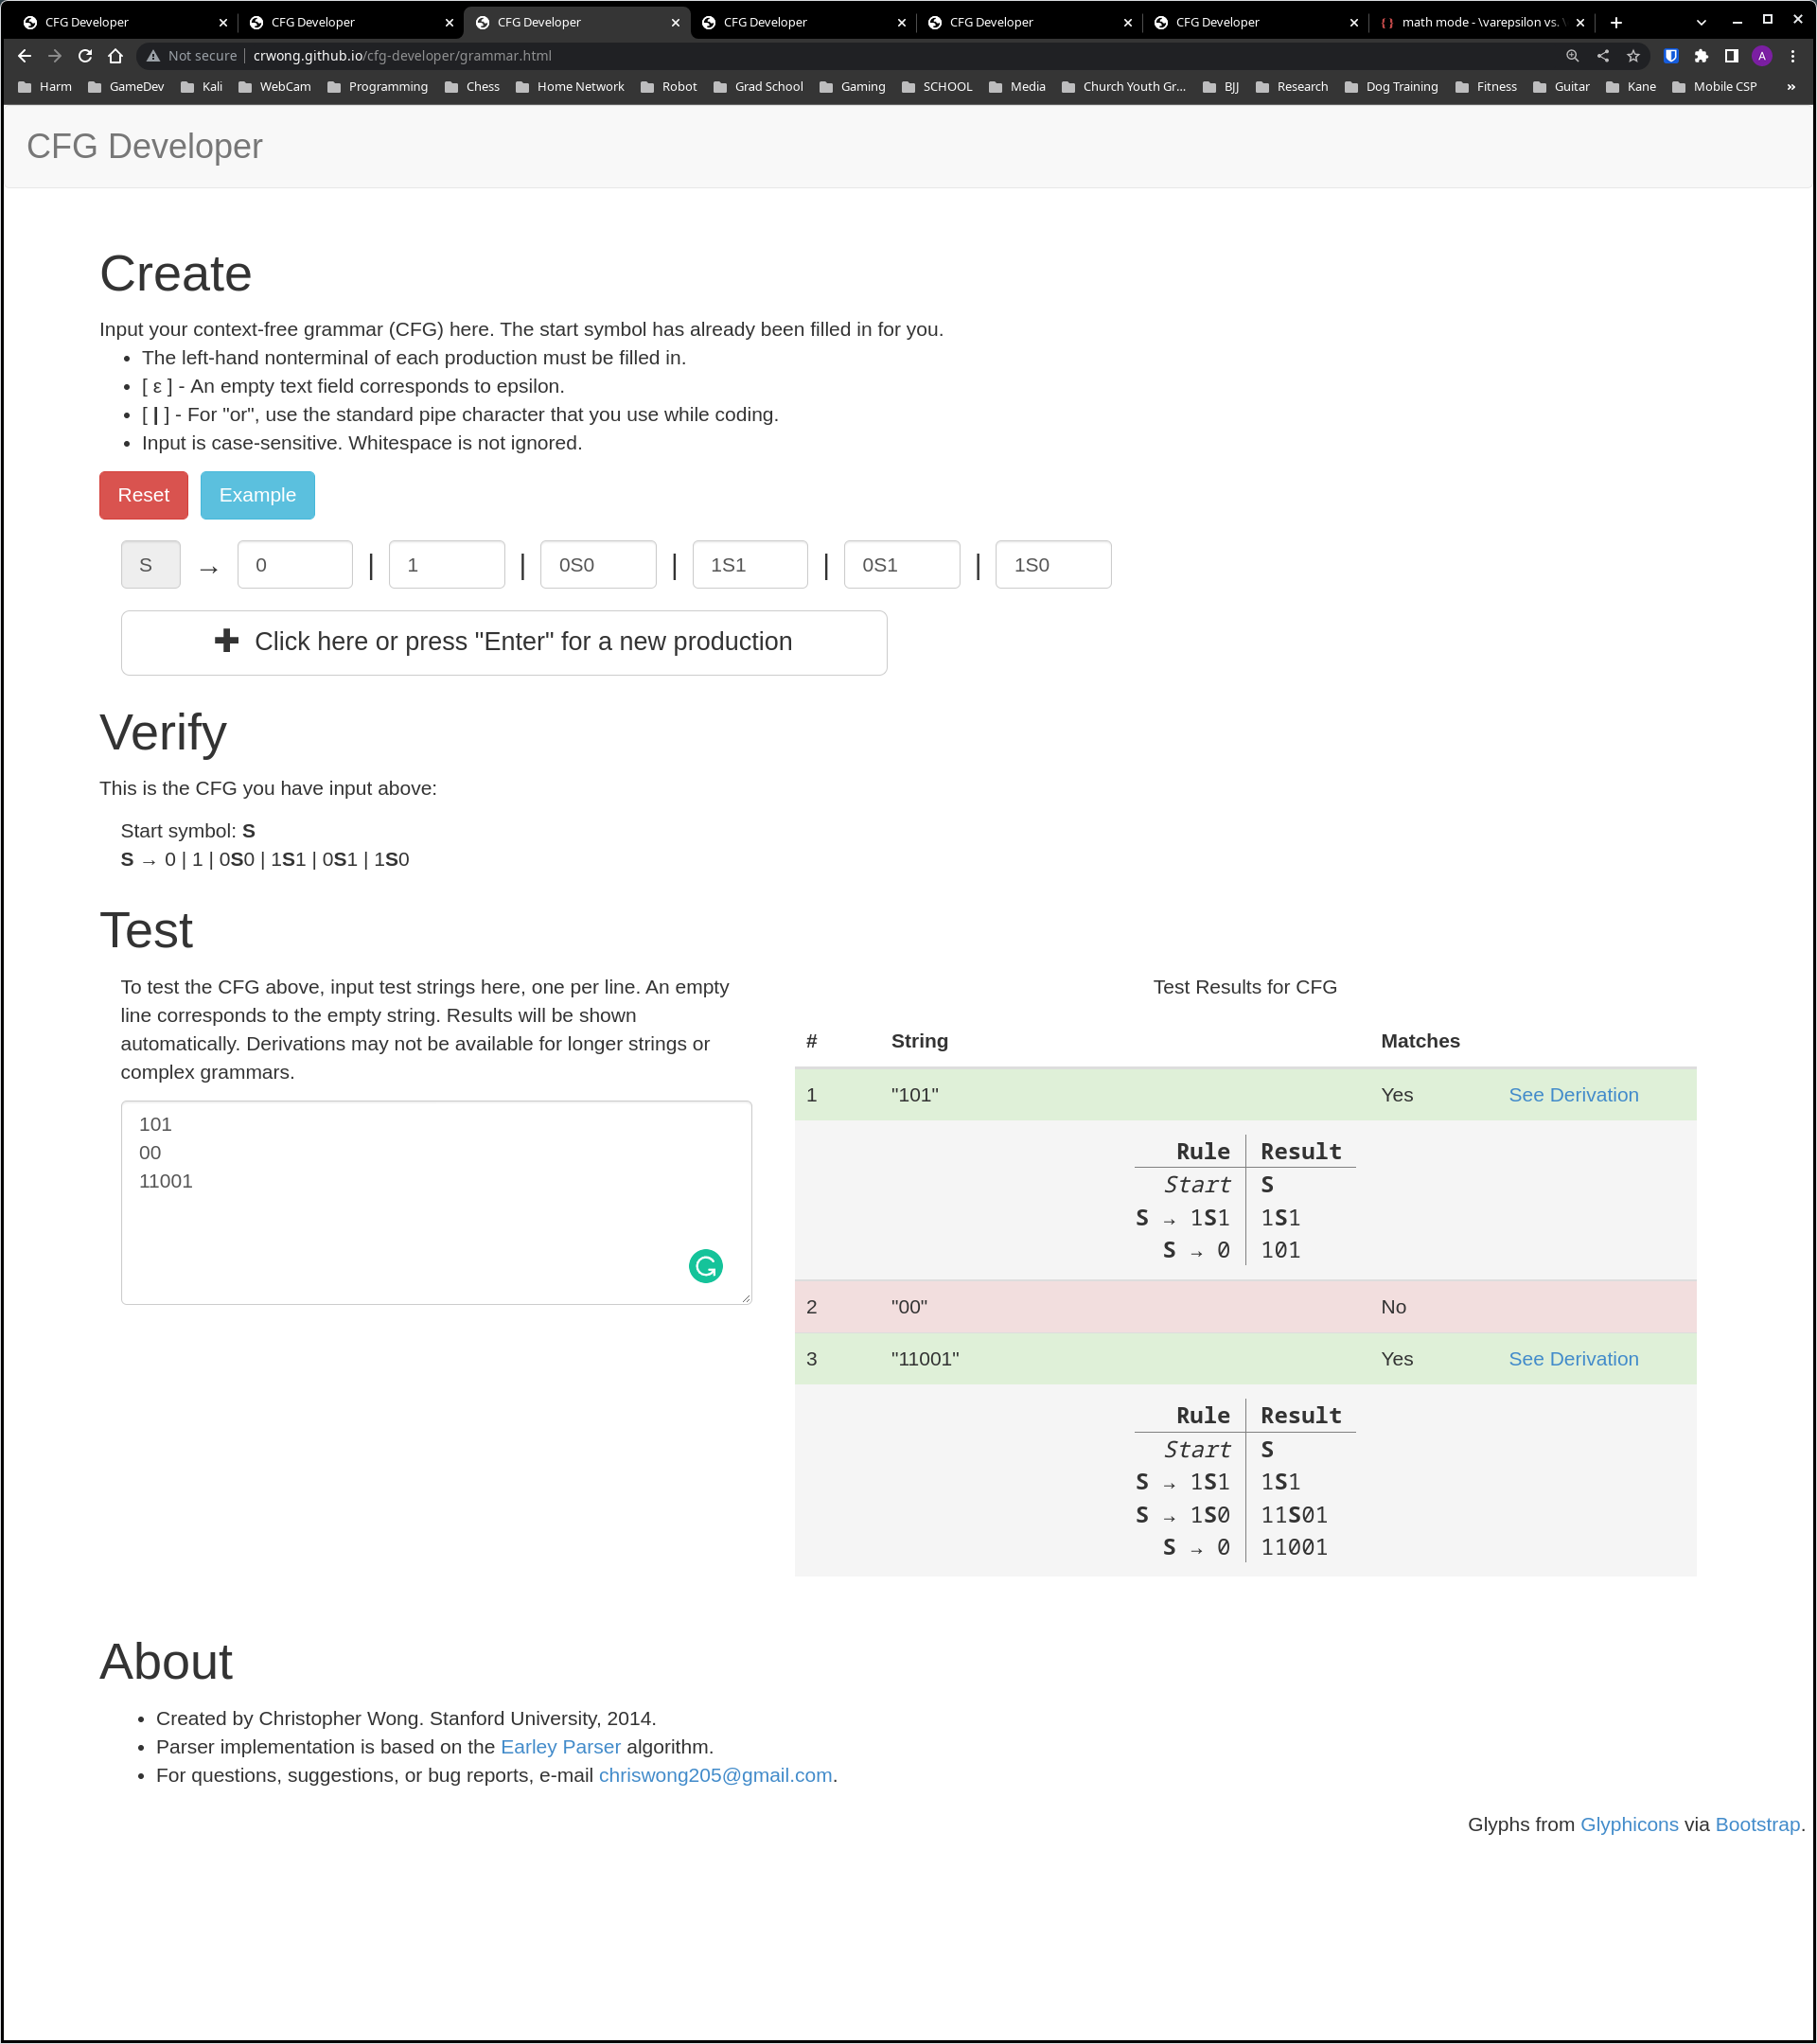
\includegraphics[width=0.4\paperwidth]{cfg_l3}\\
$L_{4}$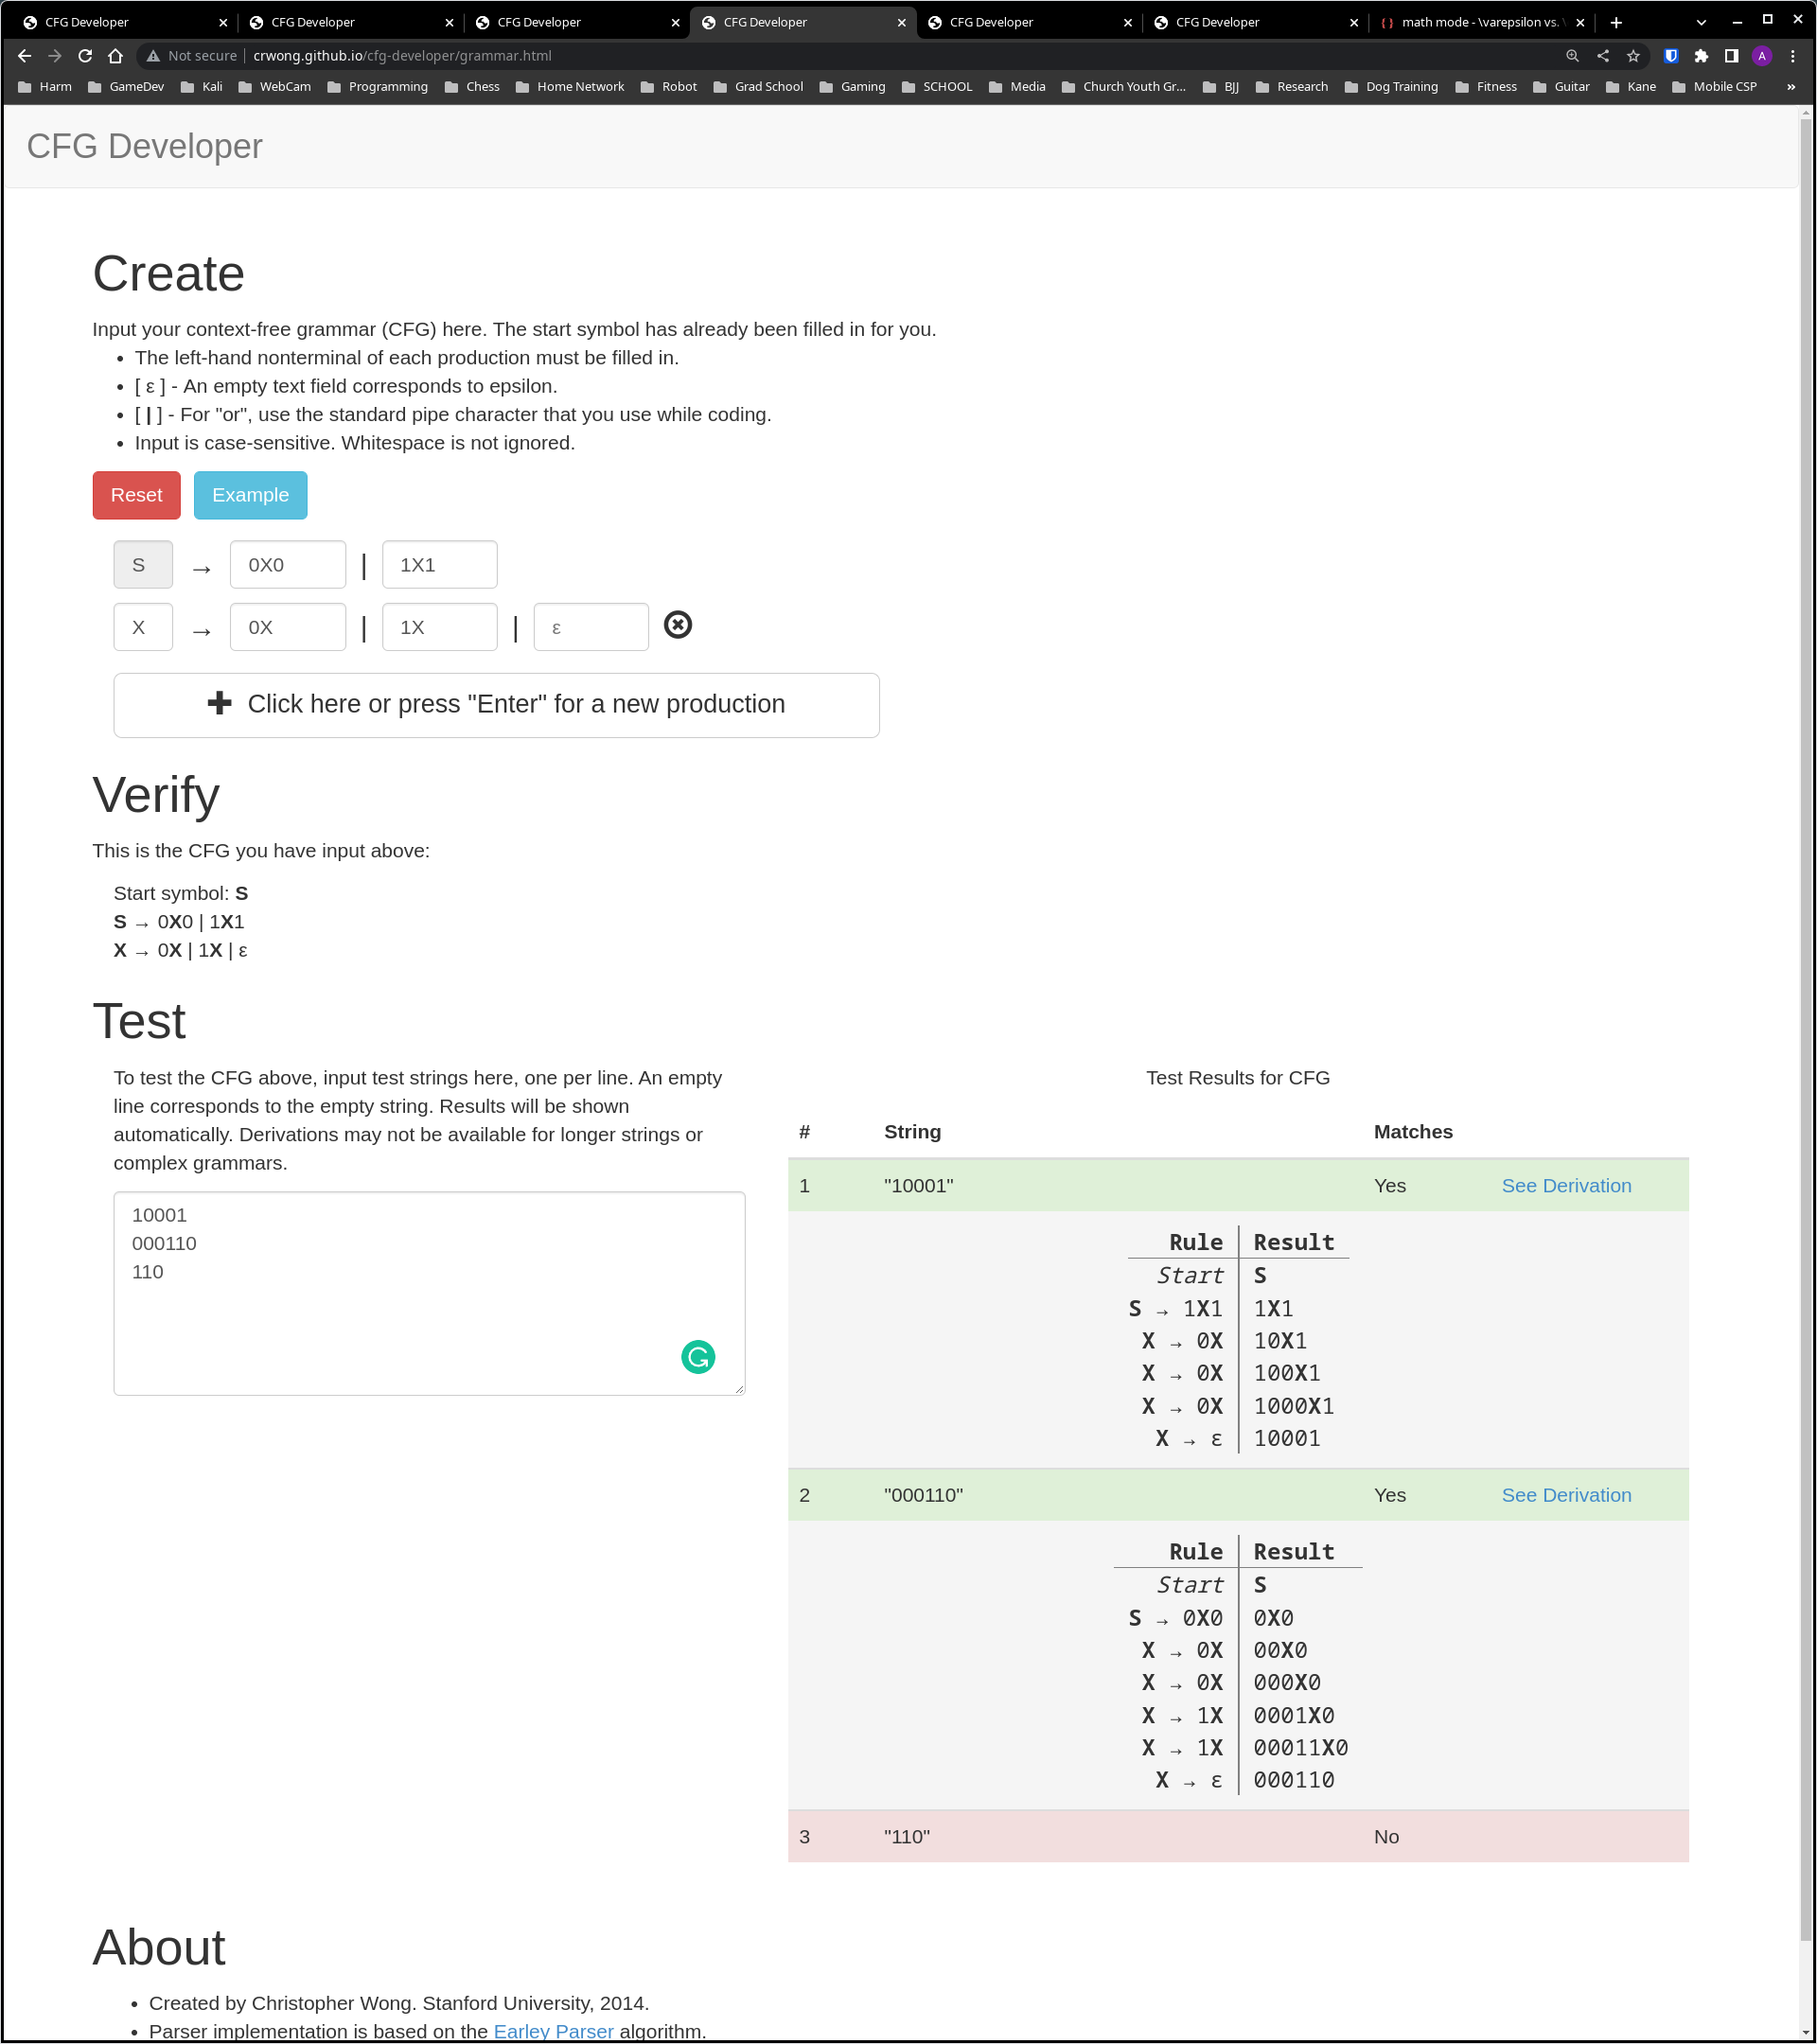
\includegraphics[width=0.4\paperwidth]{cfg_l4}\\
$L_{5}$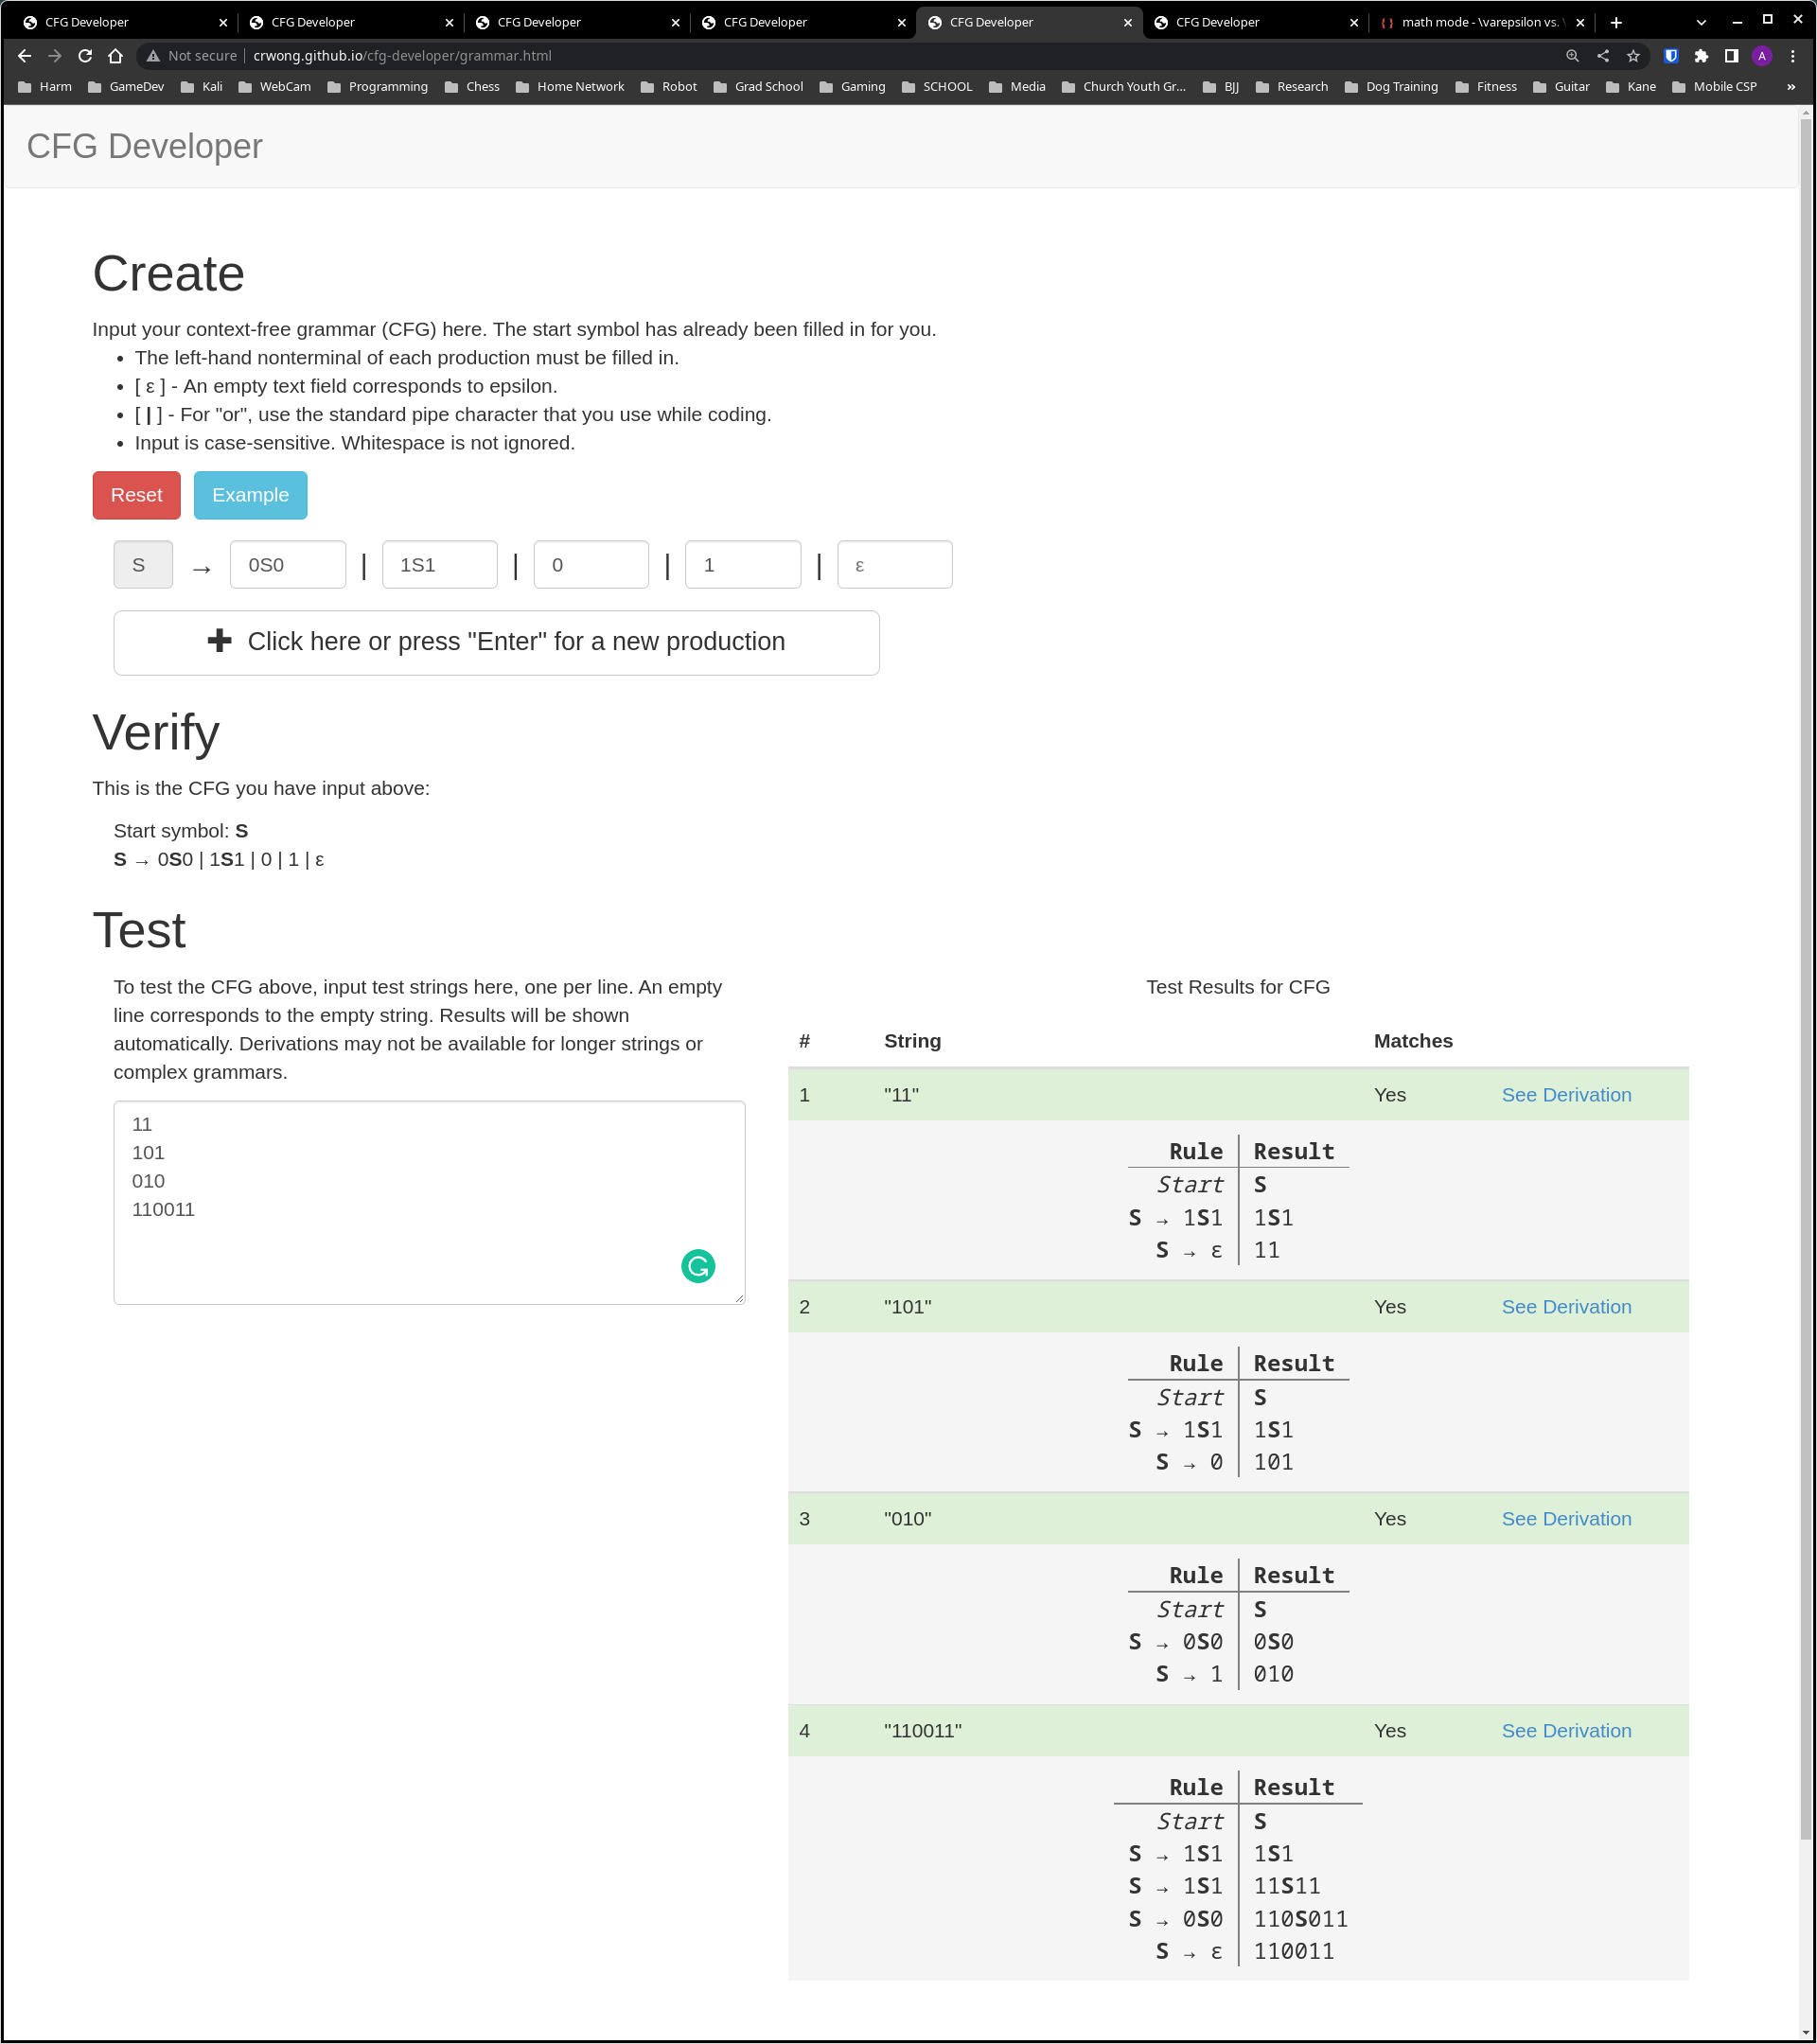
\includegraphics[width=0.4\paperwidth]{cfg_l5}\\
$L_{6}$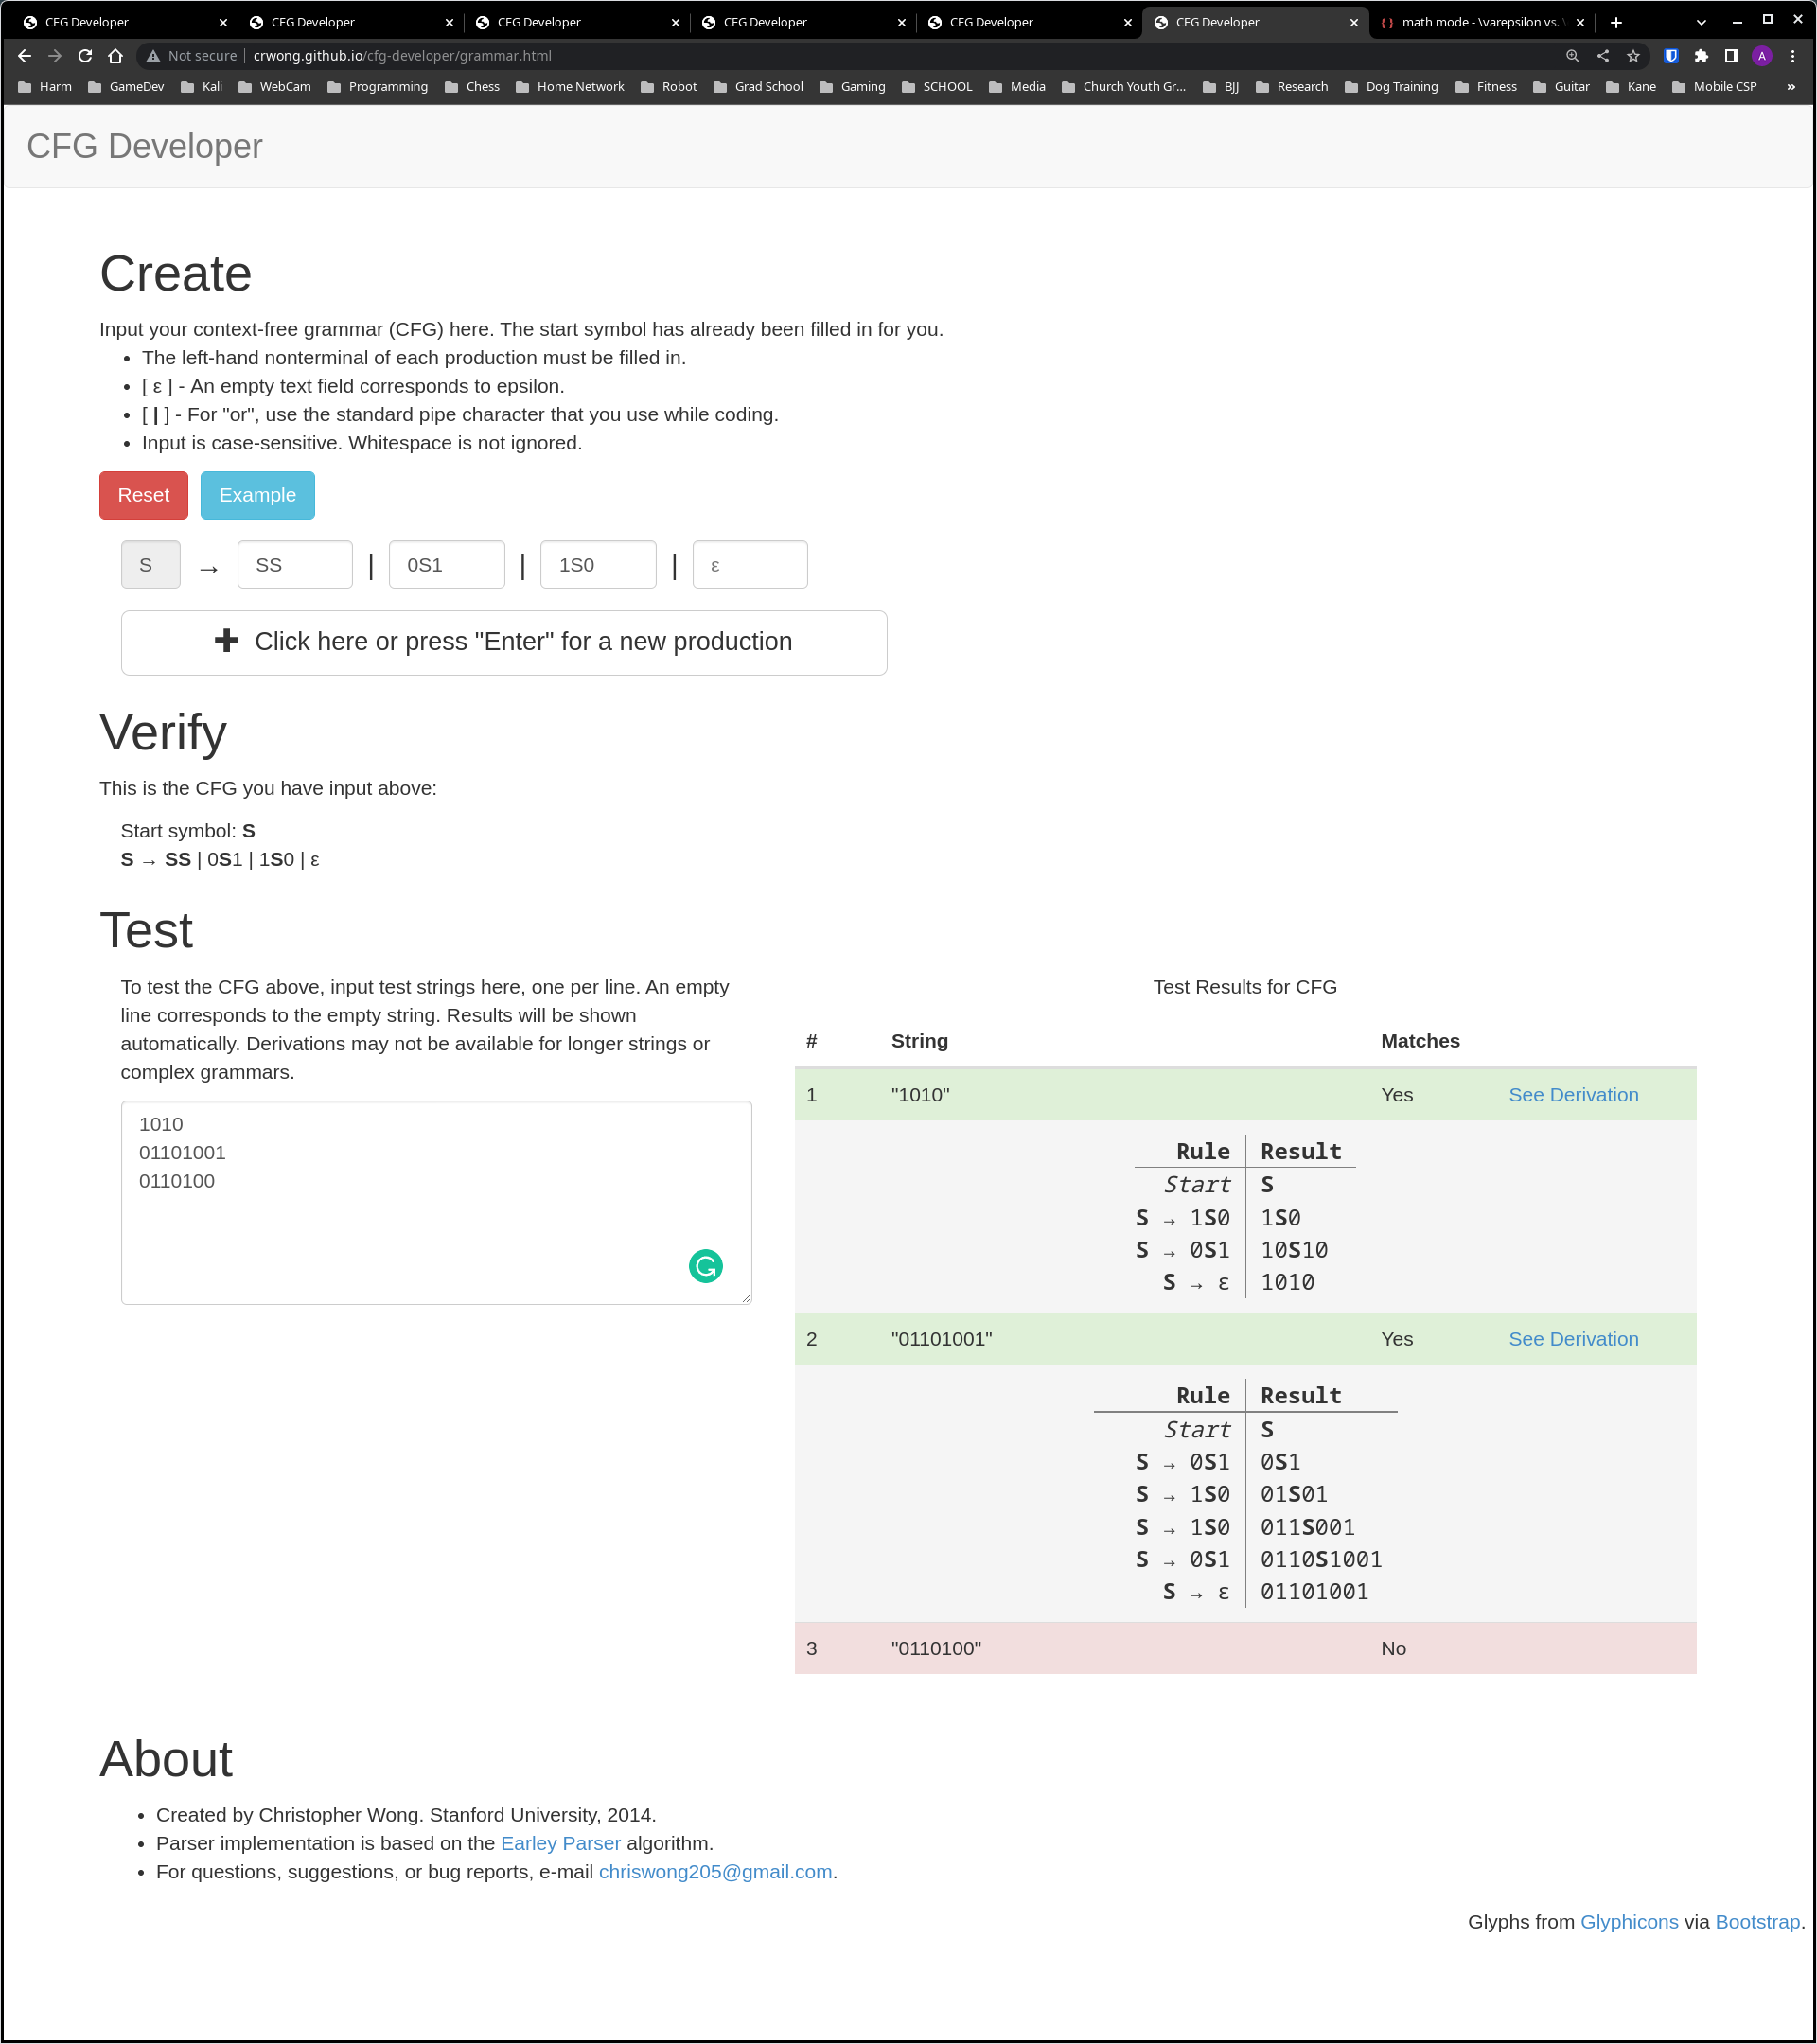
\includegraphics[width=0.4\paperwidth]{cfg_l6}

\section{Give \uline{informal descriptions} (see the solution of Exercise
2.7) and \uline{state diagrams of PDAs} for the \uline{non-regular
languages} above.}
\end{document}
